\section{Подготовка окружения}
Как уже упоминалось ранее, мы тестируем драйверы файловых систем в минималистичном UEFI-оркужении в пространстве пользователя от \cite{OpenCorePkg}. В это окружение необходимо добавить:
\begin{itemize}
	\item Эмуляцию дискового устройства: предоставить интерфейсы (\VarName{EFI\_BLOCK\_IO\_PROTOCOL}, \VarName{EFI\_DISK\_IO\_PROTOCOL}, \VarName{EFI\_DISK\_IO2\_PROTOCOL}), через которые драйвер взаимодействует с носителем
	
	\item Эмуляцию подсистемы событий UEFI: для тестирования драйверов, поддерживающих асинхронный функционал 
\end{itemize} 

\subsection{Эмулирование дискового устройства}
\begin{figure}[htbp]
	\centering % Центрирование
	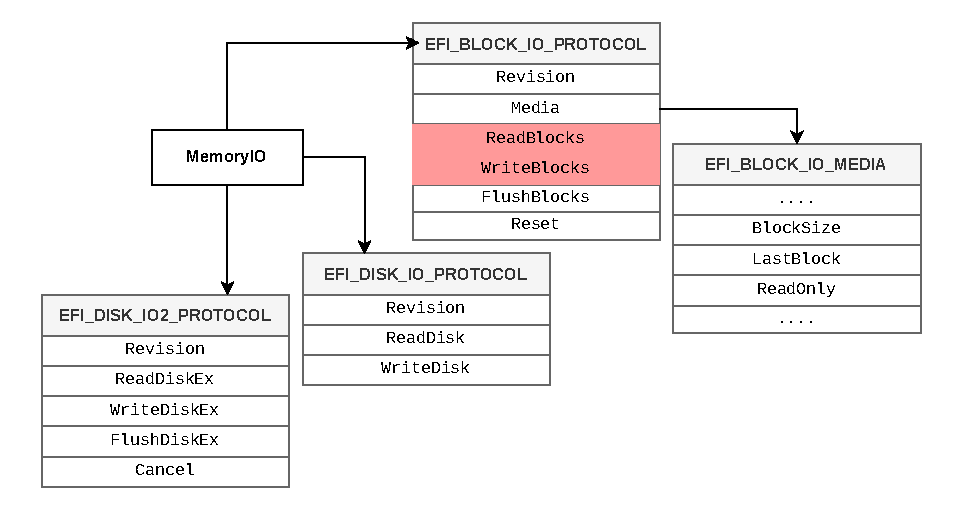
\includegraphics[width=0.8\textwidth]{MemoryIo.pdf} % Путь к файлу
	\caption{Интерфейсы, предоставляемые модулем MemoryIO} % Подпись
	\label{env:pic:memoryio} % Метка для ссылок
\end{figure}

В реальной UEFI-среде драйверы файловых систем получают доступ к носителю через стандартизированные интерфейсы (см. рисунок \ref{env:pic:memoryio})
\begin{itemize}
	\item \VarName{EFI\_BLOCK\_IO\_PROTOCOL} предоставляет доступ к устройству как к блочному, содержит информацию о носителе через \VarName{EFI\_BLOCK\_IO\_MEDIA}	
	\item \VarName{EFI\_DISK\_IO\_PROTOCOL} обеспечивает синхронный доступ к устройству как к непрерывному потоку байтов
	
	\item \VarName{EFI\_DISK\_IO2\_PROTOCOL} расширяет \VarName{EFI\_DISK\_IO\_PROTOCOL}, добавляя поддержку асинхронных операций чтения/записи/сброса
\end{itemize}
полное описание можно найти в \cite{UEFISpec}.


Для эмуляции этих интерфейсов был разработан модуль\textbf{ MemoryIO}. Его основная задача  - <<создать>> в оперативной памяти виртуальное дисковое устройство на основе тестовых данных, передаваемых libFuzzer. Модуль возвращает структуру, содержащую полные реализации всех четырех требуемых интерфейсов

Реализация функций в MemoryIO
\begin{enumerate}
	\item Синхронные операции (\FunName{ReadDisk}, \FunName{WriteDisk}) эмулируются простым копированием данных из/в буфер, соответствующий виртуальному диску в памяти. Функции \FunName{FlushBlocks} и \FunName{Reset} реализованы как заглушки, так как физического устройства не существует
	\item Асинхронные операции  (\FunName{ReadDiskEx}, \FunName{WriteDiskEx}, \FunName{FlushDiskEx})  эмулируют асинхронный ввод-вывод с использованием механизма событий UEFI:
	\begin{itemize}
		\item При вызове создается контекст задачи, содержащий тип операции, смещение, буфер данных и его размер
		\item Создается  сигнальное событие \VarName{EFI\_EVENT}, с которым ассоциируется обработчик задачи и ее контекст
		\item Создается однократный таймер EFI с небольшой задержкой (эмулирующей время выполнения операции). Этот таймер связывается с созданным событием
		\item По истечении времени таймера срабатывает событие, вызывается обработчик, который выполняет запланированную операцию, сигнализирует о завершении операции и освобождает ресурсы задачи
	\end{itemize}
	\item Функция \FunName{Cancel}  позволяет отменить все ожидающие асинхронные задачи
    \item Блочные функции (\FunName{ReadBlocks},\FunName{WriteBlocks}) не реализовывались, так как тестируемые драйверы не используют их напрямую
\end{enumerate}

После инициализации MemoryIO возвращаемые им интерфейсы передаются тестируемому драйверу файловой системы. Драйвер использует их для монтирования виртуального диска и предоставления дескриптора корневого каталога \VarName{EFI\_FILE\_PROTOCOL}, через который осуществляются все операции с файловой системой

\subsection{Эмуляция подсистемы событий UEFI Event}

Для обеспечения работы асинхронных операций и таймеров, задействованных как драйверами файловых систем, так и модулем MemoryIO, был реализован модуль \textbf{YummyEvent}. Он предоставляет программную эмуляцию ключевых функций подсистемы событий UEFI Boot Services \cite{UEFISpec}, включая:
\begin{itemize}
	 \item Создание/уничтожение событий \FunName{CreateEvent}/\FunName{CloseEvent}
	 \item Сигнализация событий \FunName{SignalEvent}
	 \item Ожидание событий \FunName{WaitForEvent}
	 \item Управление таймерами \FunName{SetTimer}
	 \item Контроль уровня привелегий \FunName{RaiseTPL}/\FunName{RestoreTPL}
	 \item Проверка состояния событий \FunName{CheckEvent}
	 \item Поддерживаемые типы событий: сигнальные, ожидающие, периодические таймеры
\end{itemize}

Особенность реализации заключается в принципе явной диспетчеризации событий. Обработка событий (включая срабатывание таймеров и вызов callback-функций) не происходит в фоновых потоках. Вместо этого она инициируется исключительно при вызове методов UEFI Event, например таких как \FunName{SignalEvent}, \FunName{WaitForEvent} или \FunName{RaiseTPL}. Такой подход обеспечивает следующие характеристики:
\begin{itemize}
	\item Обработчики событий выполняются в контексте вполняющегося кода, что эмулирует поведение прерываний в UEFI среде
	\item Отсутствие фоновой асинхронности гарантирует воспроизводимость результатов фаззинга
	\item Упрощение отладки
\end{itemize}

Для решения проблемы своевременного срабатывания таймеров введена функция \FunName{YummyEventsDispatch}. Её принудительный вызов позволяет <<продвинуть>> системное время, сработать ожидающим таймерам и обработать накопившиеся события. 
